\section{Lab 4 - Kalman filter}
\subsection{Motivation}
In this lab we are supposed to dive in to the realm of an other state estimator, Kalman filter. It is tuned based on process noise and measurment noise, and will be used to a stochastic model of the system.
Unlike the Luenberger observer which calculates a constant gain, the kalman gain is computed and varies with each timestep. This lab takes us through discretization 
of the state space system and expirementation of measurement covariance and covariance of disturbance. 

\subsection{Lab preperation}
Our first task in the lab preperation was to derive the discrete system model of the state space model.
The discrete system model is at the form \ref{eq:discrete_model} where as the matrix equations can be found in \ref{eq:discrete_matrices}.

\begin{subequations}\label{eq:discrete_model}
    \begin{align}
    x[k+1] &= A_d x[k] + B_d u[k] + \omega_d[k] \label{eq:discrete_x} \\
    y[k] &= C_d x[k] + v_d[k] \label{eq:discrete_y} \\
    \omega_d &\sim \mathcal{N}(0, Q_d), \quad v_d \sim \mathcal{N}(0, R_d) \label{eq:discrete_noise}
    \end{align}
\end{subequations}


\begin{subequations}\label{eq:discrete_matrices}
    \begin{align}
    A_d &= e^{AT} = \begin{bmatrix}
    1 & 1 & 0 & 0 & 0 & 0\\
    0 & 1 & 0 & 0 & 0 & 0\\
    0 & 0 & 1 & 1 & 0 & 0\\
    0 & 0 & 0 & 1 & 0 & 0\\
    \frac{K3}{2} & \frac{K3}{6} & 0 & 0 & 1 & 1\\
    K3 & \frac{K3}{2} & 0 & 0 & 0 & 1\\
    \end{bmatrix} \label{eq:discrete_Ad}\\
    B_d &= \int\limits_0^T e^{A\alpha} \, d\alpha \, B \ = \begin{bmatrix}
    0 & \frac{K1T^2}{2} \\
    0 & K1T \\
    \frac{K2T^2}{2} & 0 \\
    K2T & 0 \\
    0 & \frac{K1K3T^4}{24} \\
    0 & \frac{K1K3T^3}{6} \\
    \end{bmatrix} \label{eq:discrete_Bd}\\
    C_d &= C = \begin{bmatrix}
        1 & 0 & 0 & 0 & 0 & 0\\
        0 & 1 & 0 & 0 & 0 & 0\\
        0 & 0 & 1 & 0 & 0 & 0\\
        0 & 0 & 0 & 1 & 0 & 0\\
        0 & 0 & 0 & 0 & 0 & 1\\
    \end{bmatrix}\label{eq:discrete_Cd}
    \end{align}
\end{subequations}
\subsection{Hypotheses/Test plan}
For the tests we were supposed to change the Qd matrix, which has a role of specifying how much the Kalman filter should trust the model vs measurements. A small Qd 
means high trust in the measurements, while a high Qd means low trust in measurements and high in model. 
During the tests we added a step to pi/4 in the pitch reference from 3s to 8s. 
\begin{table}[h]
    \centering
    \phantomsection % Creates an anchor for the hyperlink
     % Place the label at the top of the table
        \begin{tabular}{||c c c c||} 
         \hline
         Test & Q  & Hypotheses & Result \\ [0.5ex] 
         \hline\hline
         1 & 5 & Medium noise in state est. & Noisy \\ 
         \hline
         2 & 0.1 & Low noise in state est. & Noisy \\
         \hline
         3 & 1000 & High noise in state est. & Noisy  \\ [1ex]
         \hline
        \end{tabular}
        \label{tab:testskjema_lab4}
        \caption{Test scheme lab4}
    \end{table}
\subsection{Results}
Because of the IMU (which is used to give measurements to the Kalman filter) has a lower 
sample rate than Simulink, we were needed to adjust the Kalman filter program to that. 
When there were duplicated measurements as input to the Kalman filter, we made the corrected
state estimate and error covariance to be equal to the predicted state estimate and error covariance. See \ref{eq:slow_sample}.
\begin{subequations}\label{eq:slow_sample}
    \begin{align}
    \hat{x} &= \bar{x}  \label{eq:bad_sample_x} \\
    \hat{P} &= \bar{P} \label{eq:bad_sample_p} \\
    \end{align}
\end{subequations}
The first task at the lab was to find an estimate on measurement noise. To do this we 
created two different time series, one for the helicopter laying still and one for the helicopter in the linearization point.
The estimated measurement noise used for the task corresponds to when the helicopter is stationary in its linearization point.
The resulted covariance matrices can be seen in \ref{eq:noise_est}. Rg is for helicopter on ground and Rd when helicopter in stationary linearization point.
Taking a glance at the two matrices they seem to be nearly identical, with only a few decimal difference in som covariances. 
From this it seems that it is indifferent which of them is chosen for the Kalman filter.
\begin{subequations}\label{eq:noise_est}
    \begin{align}
    R_f &=  \begin{bmatrix}
    2.9398 & -0.0135 & -0.3548 & 0.0031 & -0.0667\\
    -0.0135 &   0.0001  &  0.0016  & -0.0000  &  0.0003\\
   -0.3548  &  0.0016  &  0.0428  & -0.0004  &  0.0080\\
    0.0031  & -0.0000 &  -0.0004 &   0.0000  & -0.0001\\
   -0.0667  &  0.0003  &  0.0080 &  -0.0001  &  0.0015\\
    \end{bmatrix}\label{eq:Rg}\\
    R_d &= \begin{bmatrix}
        2.9546  & -0.0147  & -0.3545  &  0.0024   &-0.0668\\
        -0.0147 &   0.0001 &   0.0018 &  -0.0000  &  0.0003\\
        -0.3545 &   0.0018  &  0.0425 &  -0.0003  &  0.0080\\
         0.0024 &  -0.0000  & -0.0003 &   0.0000  & -0.0001\\
        -0.0668 &   0.0003  &  0.0080 &  -0.0001  &  0.0015\\
    \end{bmatrix}\label{eq:Rd}
    \end{align}
\end{subequations}

\begin{figure}[h!]
    \centering
    \subfloat[$Q_d$:5 on diagonal]{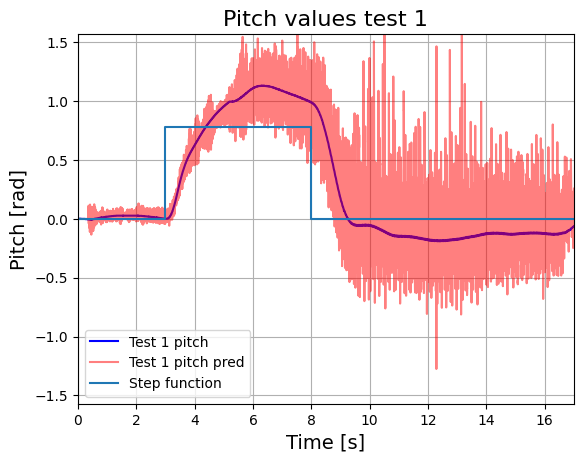
\includegraphics[width=0.3\textwidth]{figures/lab4test1pitch.png}}\hfill
    \subfloat[$Q_d$:0.1 on diagonal]{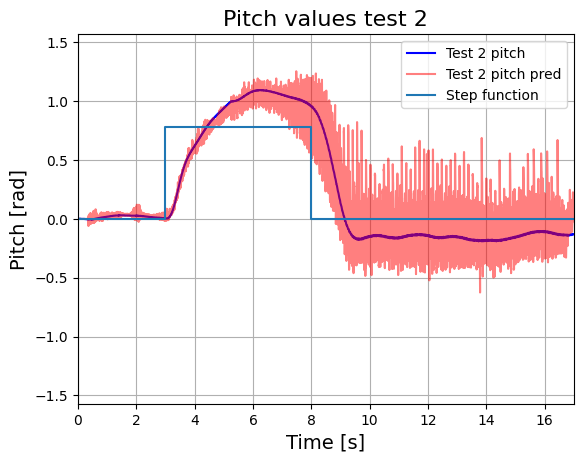
\includegraphics[width=0.3\textwidth]{figures/lab4test2pitch.png}}\hfill
    \subfloat[$Q_d$:1000 on diagonal]{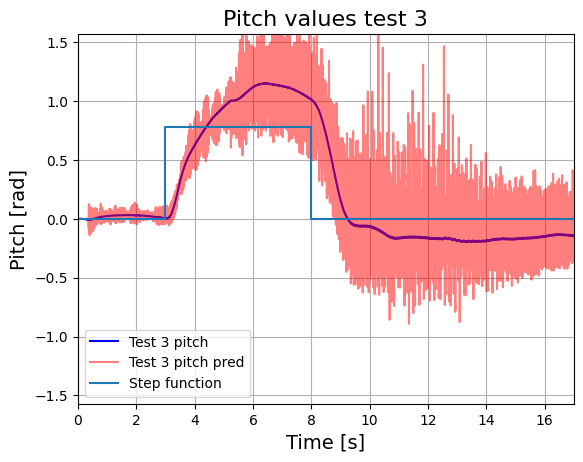
\includegraphics[width=0.3\textwidth]{figures/lab4test3pitch.png}}\hfill
    \subfloat[$Q_d$:5 on diagonal]{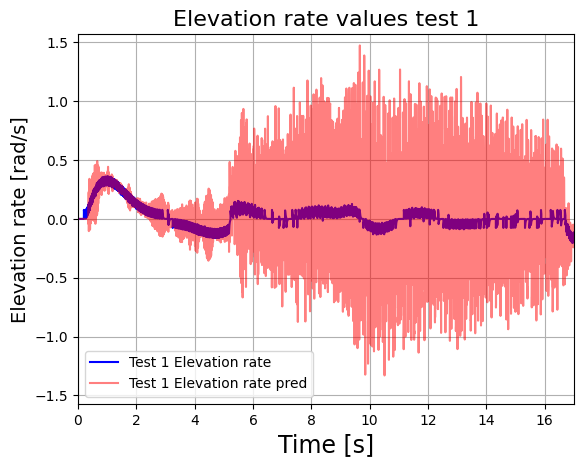
\includegraphics[width=0.3\textwidth]{figures/lab4test1ele.png}}\hfill
    \subfloat[$Q_d$:0.1 on diagonal]{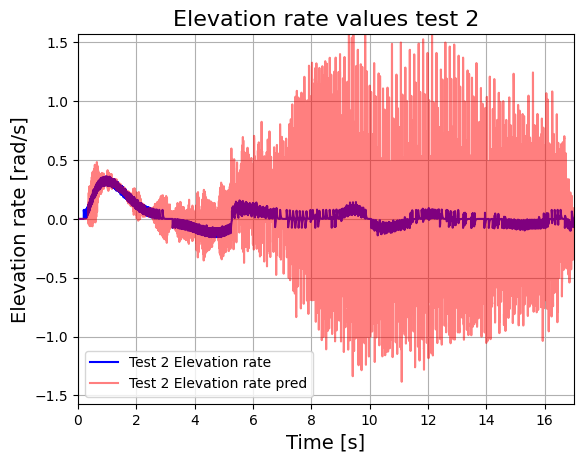
\includegraphics[width=0.3\textwidth]{figures/lab4test2ele.png}}\hfill
    \subfloat[$Q_d$:1000 on diagonal]{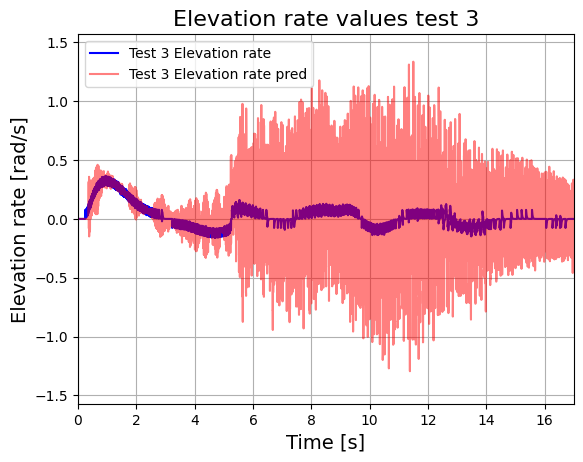
\includegraphics[width=0.3\textwidth]{figures/lab4test3ele.png}}
    \caption{Time series of pitch and elevation rate during three tests.}
    \label{fig:lab4_charts}
\end{figure}           


\subsection{Conclusion}
It was interesting to use Kalman filter to estimate the states of the system. However it seems that 
the choise of Qd indifferently affects the estimated states. It seems to be a lot of state estimation noise for all three Qd matrix tests.